% biography section
% 
% If you have an EPS/PDF photo (graphicx package needed) extra braces are
% needed around the contents of the optional argument to biography to prevent
% the LaTeX parser from getting confused when it sees the complicated
% \includegraphics command within an optional argument. (You could create
% your own custom macro containing the \includegraphics command to make things
% simpler here.)
%\begin{IEEEbiography}[{\includegraphics[width=1in,height=1.25in,clip,keepaspectratio]{mshell}}]{Michael Shell}
% or if you just want to reserve a space for a photo:
\vfill\eject

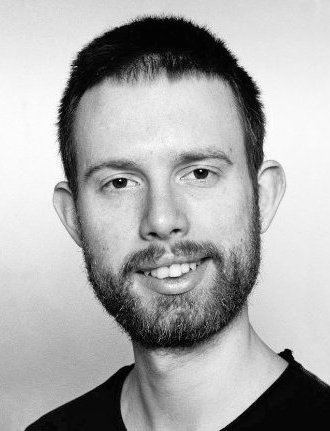
\includegraphics[width=1in,height=1.25in,clip,keepaspectratio]{img/skk.jpg}
{Stefan Krause-Kj\ae r}
is a 3rd semester Technical IT student at Aarhus University. His primary field of experience is web development and distributed systems.

% if you will not have a photo at all:
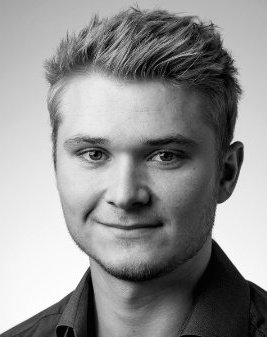
\includegraphics[width=1in,height=1.25in,clip,keepaspectratio]{img/tn.jpg}
{Theis Nickelsen}
is a 3rd semester M.Sc.Eng. IT student at Aarhus University. Since 2011 he has primarily been engaged in mobile computing and distributed systems.

% insert where needed to balance the two columns on the last page with
% biographies
%\newpage

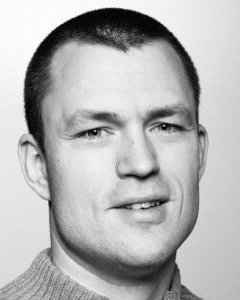
\includegraphics[width=1in,height=1.25in,clip,keepaspectratio]{img/tts.jpg}
{Thomas Thisgaard Steffensen}
is a 3rd semester M.Sc.Eng. IT student at Aarhus University. His research interests include mobile computing and distributed systems.

% You can push biographies down or up by placing
% a \vfill before or after them. The appropriate
% use of \vfill depends on what kind of text is
% on the last page and whether or not the columns
% are being equalized.

%\vfill

% Can be used to pull up biographies so that the bottom of the last one
% is flush with the other column.
%\enlargethispage{-5in}
